% Figure 1 of docs/exposition.md: the strings of all columns, and the address
% inputs, cells and outward pointers of a winning column. Adapted from
% docs/figures/expert_column.tex (same palette and bit
% cells), with the pointers routed clear of the address labels.
% Build with tools/render_papers.py.
\documentclass[tikz,border=4pt]{standalone}
% Shared TikZ style for the figures of docs/exposition.md.
% Palette and bit cells follow docs/figures/expert_column.tex.
\usepackage{amsmath,amssymb}
\usetikzlibrary{arrows.meta,positioning,calc,decorations.pathreplacing}
\definecolor{one}{RGB}{226,232,240}
\definecolor{zero}{RGB}{40,40,40}
\definecolor{win}{RGB}{176,58,46}
\definecolor{addr}{RGB}{40,90,150}
\definecolor{lose}{RGB}{110,110,110}
\tikzset{
  bit/.style={draw=black!60, minimum width=4.4mm, minimum height=4.4mm,
              inner sep=0pt, font=\scriptsize},
  onebit/.style={bit, fill=one},
  zerobit/.style={bit, fill=zero, text=white},
  cell/.style={draw=black!50, fill=white, minimum width=10mm,
               minimum height=4.2mm, inner sep=0pt, font=\scriptsize},
  >={Stealth[length=2.2mm]}}

% \boardcolumn{name}{x}{b1}{b2}{b3}{b4}{address text}
% Draws X_name as four bits at height 0 starting at x, the address inputs
% below, and the four cells 00,01,10,11 named <name>c00 ... <name>c11.
\newcommand{\boardcolumn}[7]{%
  \node[anchor=east, font=\small] at (#2-0.05,0) {$X_{#1}$};
  \foreach \c/\b in {1/#3,2/#4,3/#5,4/#6} {
    \ifnum\b=0
      \node[zerobit] (x#1-\c) at (#2+0.46*\c-0.23,0) {0};
    \else
      \node[onebit] (x#1-\c) at (#2+0.46*\c-0.23,0) {1};
    \fi}
  \node[font=\scriptsize, align=center, addr, anchor=north] (adr#1)
    at (#2+0.92,-0.38) {#7};
  \foreach \s/\k in {00/0,01/1,10/2,11/3} {
    \node[cell] (#1c\s) at (#2+0.92,-1.62-0.5*\k) {$B_{#1,\s}$};}
}

\begin{document}
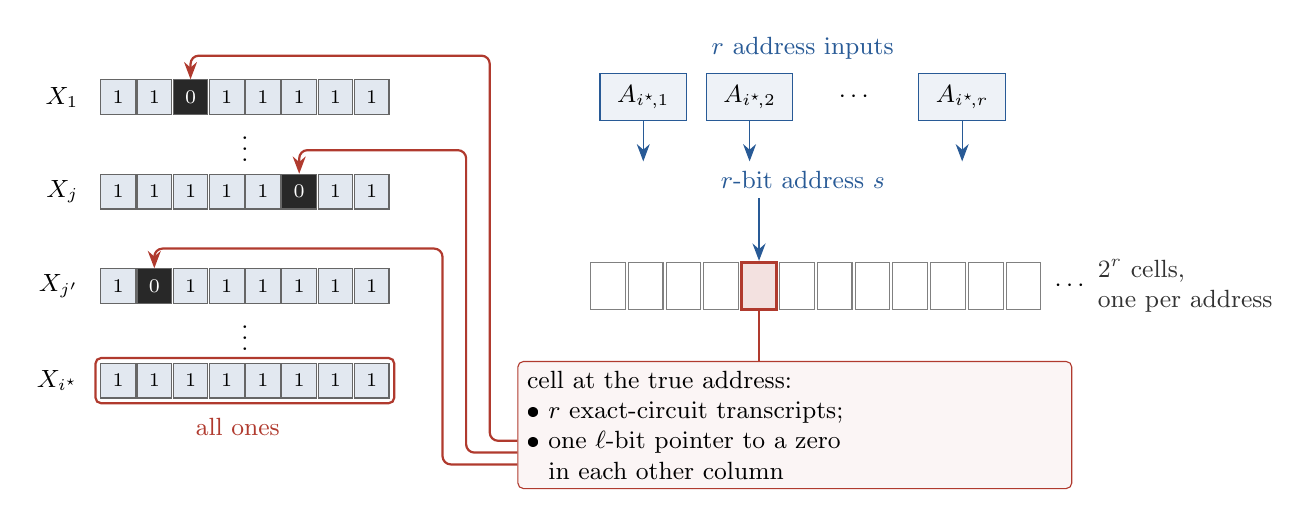
\begin{tikzpicture}[font=\small]
% ---- the strings X_j, rows of m = 8 bits --------------------------------
\newcommand{\strip}[4]{% y, label, zero position (0 = none), name
  \node[anchor=east] at (-0.15,#1) {#2};
  \foreach \c in {1,...,8} {
    \ifnum\c=#3
      \node[zerobit] (#4\c) at (0.46*\c-0.23,#1) {0};
    \else
      \node[onebit] (#4\c) at (0.46*\c-0.23,#1) {1};
    \fi}}
\strip{3.0}{$X_1$}{3}{a}
\node at (1.84,2.45) {$\vdots$};
\strip{1.8}{$X_{j}$}{6}{b}
\strip{0.6}{$X_{j'}$}{2}{c}
\node at (1.84,0.05) {$\vdots$};
\strip{-0.6}{$X_{i^\star}$}{0}{w}
\draw[win, thick, rounded corners=2pt] ($(w1.south west)+(-0.06,-0.06)$)
   rectangle ($(w8.north east)+(0.06,0.06)$);
\node[win, font=\small, anchor=north, align=center] at (1.75,-0.95)
  {all ones};
% ---- the winner's address instances -------------------------------------
\begin{scope}[shift={(6.9,3.0)}]
  \foreach \h/\lab in {0/{A_{i^\star\!,1}},1/{A_{i^\star\!,2}},3/{A_{i^\star\!,r}}} {
    \node[draw=addr, fill=addr!8, minimum width=11mm, minimum height=6mm,
          font=\small] (A\h) at (1.35*\h,0) {$\lab$};}
  \node at (2*1.35,0) {$\cdots$};
  \node[font=\small, addr, anchor=south] at (1.35*1.5,0.36)
    {$r$ address inputs};
  \node[font=\small, addr] (s) at (1.35*1.5,-1.05)
    {$r$-bit address $s$};
  \foreach \h in {0,1,3} \draw[->, addr] (A\h.south) -- (A\h.south |- s.north);
\end{scope}
% ---- the cell array B_{i*,s}, s in {0,1}^r ------------------------------
\begin{scope}[shift={(6.45,0.6)}]
  \foreach \c in {0,...,11} {
    \ifnum\c=4
      \node[draw=win, very thick, fill=win!15, minimum width=4.4mm,
            minimum height=6mm, inner sep=0pt] (cell\c) at (0.48*\c,0) {};
    \else
      \node[draw=black!50, fill=white, minimum width=4.4mm,
            minimum height=6mm, inner sep=0pt] (cell\c) at (0.48*\c,0) {};
    \fi}
  \node[anchor=west] at (5.55,0) {$\cdots$};
  \node[font=\small, black!80, anchor=west, align=left] at (6.1,0)
    {$2^r$ cells,\\one per address};
\end{scope}
\draw[->, addr, thick] (s.south -| cell4.north) -- (cell4.north);
% ---- what the selected cell holds ---------------------------------------
\node[draw=win, fill=win!5, rounded corners=2pt, align=left, font=\small,
      anchor=north west, text width=68mm] (content) at (5.3,-0.35)
  {cell at the true address:\\
   \textbullet\ $r$ exact-circuit transcripts;\\
   \textbullet\ one $\ell$-bit pointer to a zero\\
   \phantom{\textbullet\ }in each other column};
\draw[win] (cell4.south) -- (cell4.south |- content.north);
% ---- outward pointers, routed through the lanes between the blocks ------
% The lane nearest the box serves the top row, so no two pointers cross.
\draw[->, win, thick, rounded corners=3pt]
  ($(content.west)+(0,-0.2)$) -- ($(content.west)+(-0.35,-0.2)$)
  |- ($(a3.north)+(0,0.3)$) -- (a3.north);
\draw[->, win, thick, rounded corners=3pt]
  ($(content.west)+(0,-0.35)$) -- ($(content.west)+(-0.65,-0.35)$)
  |- ($(b6.north)+(0,0.3)$) -- (b6.north);
\draw[->, win, thick, rounded corners=3pt]
  ($(content.west)+(0,-0.5)$) -- ($(content.west)+(-0.95,-0.5)$)
  |- ($(c2.north)+(0,0.25)$) -- (c2.north);
\end{tikzpicture}
\end{document}
